\documentclass[12pt]{article}

\usepackage[a4paper,margin=1in]{geometry}
\usepackage{amsmath,amssymb,amsthm}
\usepackage{tikz}
\usepackage{enumitem}
\usepackage{xcolor}

\setlength{\parindent}{0pt}
\setlength{\parskip}{0.75em}

\newtheorem{definition}{Definition}
\newtheorem{remark}{Remark}
\newtheorem{example}{Example}

\title{Lecture 11 Supplement: Disease Exists on Day 2}
\author{MA4034 -- Time Series and Stochastic Processes}
\date{}

\begin{document}

\maketitle

\section{What This Question Is About}

We are studying the early spread of a disease using a \textbf{branching process}.

Let
\[
Z_n=\text{number of infected individuals on day }n.
\]

The question asks:

\begin{center}
\textit{What is the probability that the disease still exists on day 2?}
\end{center}

That means we want
\[
P(Z_2>0).
\]

It is usually easier to first find the opposite event:
\[
P(Z_2=0),
\]
which means the disease is extinct by day 2.

Then
\[
P(Z_2>0)=1-P(Z_2=0).
\]

\section{Offspring Distribution}

In this disease example:

\begin{itemize}
    \item Each infected person meets a random number of people.
    \item The number of people met has mean 10.
    \item Each person met becomes infected with probability \(p\).
\end{itemize}

When \(p=0.2\), the expected number of new infections caused by one infected person is
\[
10p=10(0.2)=2.
\]

So the number of people infected by one person is
\[
X\sim \operatorname{Poisson}(2).
\]

Here \(X\) is called the \textbf{offspring random variable}.

\begin{definition}[Offspring Random Variable]
In a branching process, the offspring random variable \(X\) is the number of new individuals produced by one current individual.

In this disease example, \(X\) is the number of new infected people produced by one infected person.
\end{definition}

\section{Probability Generating Function}

The probability generating function, or PGF, of \(X\) is
\[
G(s)=E(s^X).
\]

For a Poisson random variable with mean \(\lambda\),
\[
G(s)=e^{\lambda(s-1)}.
\]

Since here \(\lambda=2\),
\[
G(s)=e^{2(s-1)}.
\]

\section{Why Does \(G(0)\) Give Extinction After One Day?}

Remember:
\[
G(s)=E(s^X).
\]

If \(s=0\), then
\[
G(0)=E(0^X).
\]

Now observe:
\[
0^X=
\begin{cases}
1, & X=0,\\
0, & X\geq 1.
\end{cases}
\]

Therefore,
\[
E(0^X)=P(X=0).
\]

So
\[
G(0)=P(X=0).
\]

In words:

\begin{center}
\fbox{\parbox{0.85\textwidth}{
\[
G(0)=\text{probability that one infected person infects nobody.}
\]
}}
\end{center}

Since we start with one infected person,
\[
G(0)=P(Z_1=0).
\]

That is the probability that the disease is extinct after day 1.

\section{Calculating \(G(0)\)}

Since
\[
G(s)=e^{2(s-1)},
\]
we get
\[
G(0)=e^{2(0-1)}=e^{-2}.
\]

So
\[
P(Z_1=0)=e^{-2}.
\]

Numerically,
\[
e^{-2}\approx 0.1353.
\]

This means there is about a \(13.53\%\) chance that the original infected person infects nobody.

\section{Why Does \(G(G(0))\) Give Extinction After Day 2?}

This is the most important idea.

The disease is extinct by day 2 if all infected people in day 1 produce zero infected people in day 2.

But the number of infected people on day 1 is random.

There may be:
\[
0,1,2,3,\ldots
\]
infected people on day 1.

Suppose there are \(k\) infected people on day 1.

For the disease to be extinct on day 2:

\begin{itemize}
    \item person 1 must infect nobody,
    \item person 2 must infect nobody,
    \item \(\ldots\)
    \item person \(k\) must infect nobody.
\end{itemize}

Each person infects nobody with probability
\[
G(0).
\]

So if there are \(k\) people on day 1, the probability that all of them infect nobody is
\[
\bigl(G(0)\bigr)^k.
\]

But \(k=Z_1\) is random. Therefore we take expectation:
\[
P(Z_2=0)=E\left[\bigl(G(0)\bigr)^{Z_1}\right].
\]

By the definition of PGF,
\[
E(s^{Z_1})=G(s).
\]

Here \(s=G(0)\). Hence,
\[
P(Z_2=0)=G(G(0)).
\]

\begin{center}
\fbox{\parbox{0.85\textwidth}{
\[
G(G(0))=\text{probability that the disease is extinct by day 2.}
\]
}}
\end{center}

\section{Step-by-Step Calculation}

We already found
\[
G(0)=e^{-2}.
\]

Now calculate
\[
G_2(0)=G(G(0)).
\]

Substitute \(G(0)=e^{-2}\):
\[
G_2(0)=G(e^{-2}).
\]

Since
\[
G(s)=e^{2(s-1)},
\]
put \(s=e^{-2}\):
\[
G(e^{-2})=e^{2(e^{-2}-1)}.
\]

Therefore,
\[
P(Z_2=0)=e^{2(e^{-2}-1)}.
\]

Numerically,
\[
P(Z_2=0)\approx 0.18.
\]

So the probability that the disease still exists on day 2 is
\[
P(Z_2>0)=1-P(Z_2=0).
\]

Thus,
\[
P(Z_2>0)=1-e^{2(e^{-2}-1)}.
\]

Numerically,
\[
P(Z_2>0)\approx 1-0.18=0.82.
\]

So
\[
\boxed{P(\text{disease still exists on day 2})\approx 0.82.}
\]

\section{Small Diagram of the Idea}

\begin{center}
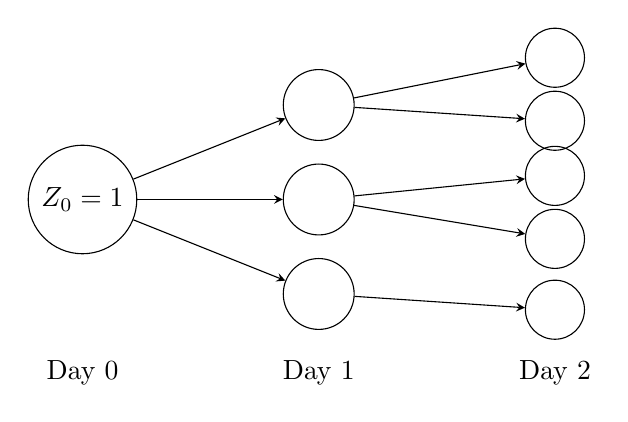
\begin{tikzpicture}[>=stealth, node distance=1.7cm]
    \node[circle,draw,minimum size=0.9cm] (z0) at (0,0) {\(Z_0=1\)};
    \node[circle,draw,minimum size=0.9cm] (a) at (3,1.2) {};
    \node[circle,draw,minimum size=0.9cm] (b) at (3,0) {};
    \node[circle,draw,minimum size=0.9cm] (c) at (3,-1.2) {};

    \node[circle,draw,minimum size=0.75cm] (a1) at (6,1.8) {};
    \node[circle,draw,minimum size=0.75cm] (a2) at (6,1.0) {};
    \node[circle,draw,minimum size=0.75cm] (b1) at (6,0.3) {};
    \node[circle,draw,minimum size=0.75cm] (b2) at (6,-0.5) {};
    \node[circle,draw,minimum size=0.75cm] (c1) at (6,-1.4) {};

    \draw[->] (z0) -- (a);
    \draw[->] (z0) -- (b);
    \draw[->] (z0) -- (c);
    \draw[->] (a) -- (a1);
    \draw[->] (a) -- (a2);
    \draw[->] (b) -- (b1);
    \draw[->] (b) -- (b2);
    \draw[->] (c) -- (c1);

    \node at (0,-2.2) {Day 0};
    \node at (3,-2.2) {Day 1};
    \node at (6,-2.2) {Day 2};
\end{tikzpicture}
\end{center}

The number of people on day 1 is random. To be extinct by day 2, every day-1 infected person must produce zero new infections.

\section{Analogy}

Think of the disease like a candle flame.

\begin{itemize}
    \item On day 0, there is one flame.
    \item On day 1, that flame may light some new candles.
    \item On day 2, each of those new candles may light more candles.
\end{itemize}

\[
G(0)
\]
means the first flame lights no new candles.

\[
G(G(0))
\]
means that after the first round of flames, all of the flames in the next round also fail to light new candles.

\section{Common Mistake}

Do not say:
\[
G(0)=\text{probability disease exists on day 1}.
\]

That is incorrect.

Instead:
\[
G(0)=P(Z_1=0)=\text{probability disease is extinct by day 1}.
\]

Similarly:
\[
G(G(0))=P(Z_2=0)=\text{probability disease is extinct by day 2}.
\]

So:
\[
1-G(G(0))=P(Z_2>0)=\text{probability disease still exists on day 2}.
\]

\section{Practice Questions With Answers}

\subsection*{Question 1}

Suppose \(X\sim \operatorname{Poisson}(3)\). Write the PGF \(G(s)\).

\textbf{Answer.}

For a Poisson random variable with mean \(\lambda\),
\[
G(s)=e^{\lambda(s-1)}.
\]

Here \(\lambda=3\), so
\[
\boxed{G(s)=e^{3(s-1)}.}
\]

\subsection*{Question 2}

Suppose \(X\sim \operatorname{Poisson}(2)\). Find the probability that a single infected person infects nobody.

\textbf{Answer.}

The probability that the person infects nobody is
\[
P(X=0).
\]

Using the PGF,
\[
P(X=0)=G(0).
\]

Since
\[
G(s)=e^{2(s-1)},
\]
we get
\[
G(0)=e^{2(0-1)}=e^{-2}.
\]

Therefore,
\[
\boxed{P(X=0)=e^{-2}\approx 0.1353.}
\]

\subsection*{Question 3}

For the same process with \(G(s)=e^{2(s-1)}\), find \(P(Z_2=0)\).

\textbf{Answer.}

We use
\[
P(Z_2=0)=G(G(0)).
\]

First,
\[
G(0)=e^{-2}.
\]

Then
\[
G(G(0))=G(e^{-2}).
\]

Since
\[
G(s)=e^{2(s-1)},
\]
we get
\[
G(e^{-2})=e^{2(e^{-2}-1)}.
\]

Therefore,
\[
\boxed{P(Z_2=0)=e^{2(e^{-2}-1)}\approx 0.18.}
\]

\subsection*{Question 4}

Using Question 3, find the probability that the disease still exists on day 2.

\textbf{Answer.}

Disease still exists on day 2 means
\[
Z_2>0.
\]

So
\[
P(Z_2>0)=1-P(Z_2=0).
\]

From Question 3,
\[
P(Z_2=0)=e^{2(e^{-2}-1)}.
\]

Therefore,
\[
P(Z_2>0)=1-e^{2(e^{-2}-1)}.
\]

Numerically,
\[
\boxed{P(Z_2>0)\approx 0.82.}
\]

\subsection*{Question 5}

Suppose \(G(s)=0.4+0.6s^2\). Find \(P(Z_1=0)\) and \(P(Z_2=0)\).

\textbf{Answer.}

First,
\[
P(Z_1=0)=G(0).
\]

So
\[
G(0)=0.4+0.6(0)^2=0.4.
\]

Thus,
\[
\boxed{P(Z_1=0)=0.4.}
\]

Next,
\[
P(Z_2=0)=G(G(0)).
\]

Since \(G(0)=0.4\),
\[
P(Z_2=0)=G(0.4).
\]

Now
\[
G(0.4)=0.4+0.6(0.4)^2.
\]

So
\[
G(0.4)=0.4+0.6(0.16)=0.4+0.096=0.496.
\]

Therefore,
\[
\boxed{P(Z_2=0)=0.496.}
\]

\subsection*{Question 6}

In words, explain why \(G(G(0))\) appears instead of just \(G(0)^2\).

\textbf{Answer.}

\(G(0)^2\) would be correct only if we knew there were exactly two infected people on day 1.

But the number of infected people on day 1 is random.

There could be \(0,1,2,3,\ldots\) infected people on day 1.

So we must average over all possible values of \(Z_1\). The PGF does this averaging automatically:
\[
E\left[\bigl(G(0)\bigr)^{Z_1}\right]=G(G(0)).
\]

That is why the correct expression is
\[
\boxed{G(G(0)),}
\]
not \(G(0)^2\).

\section{Summary}

\begin{itemize}
    \item \(G(s)\) is the PGF of the number of new infections caused by one infected person.
    \item \(G(0)=P(Z_1=0)\), the probability the disease is extinct after one day.
    \item \(G(G(0))=P(Z_2=0)\), the probability the disease is extinct after two days.
    \item \(1-G(G(0))=P(Z_2>0)\), the probability the disease still exists on day 2.
\end{itemize}

\end{document}
